% Notes on the writing of the Master Thesis
% Book: How to Write a Lot, Paul Silvia, 2nd Edition
% Book: Getting Things Done, David Allen
%
%
% Mögliche Abgrenzung von anderen: Den hybriden Ansatz von SBST mit DSE verwenden, 
% so wie im Paper von Baars et al.
%
% Mögliche weitere Evaluation: Vergleiche die Coverage von generierten Tests zu der 
% Coverage von manuell geschriebenen Tests von Entwicklern in evaluierten Programmen.
% 

\documentclass{article}
% Please do not change this options...
\usepackage[a4paper, total={6in, 10in}]{geometry}
\usepackage{todonotes}
\usepackage{float}
\usepackage{amsmath}
\usepackage[T1]{fontenc}
\usepackage[shortlabels]{enumitem}
\makeatletter
\newcommand\BeraMonottfamily{%
  \def\fvm@Scale{0.85}% scales the font down
  \fontfamily{fvm}\selectfont% selects the Bera Mono font
}
\makeatother
\usepackage{acronym}
\usepackage{listings}
\lstset{
  numbers=left,
  xleftmargin=2.5em,
  framexleftmargin=2.5em,
  frame=,
  stepnumber=1,    
  firstnumber=1,
  numberfirstline=true,
  basicstyle=\BeraMonottfamily,
  identifierstyle=,
  stringstyle=\ttfamily,
  %keywordstyle=\color{OliveGreen},
  keywordstyle=,
  showstringspaces=false
}

\usepackage{graphicx}
\graphicspath{ {./img/} }

\begin{document}
\title{Exposé: Search-based Test Suite Generation for Rust}
\author{Vsevolod Tymofyeyev}
\date{\today}
\maketitle

\section{Motivation}
In the programming language world, there are two major sides. There are low-level languages that offer better performance at the expense of security and high-level languages that provide security for programmers through certain constructs such as garbage collection, which lead to runtime overhead. The young programming language Rust tries to combine the good from both. This statically typed language for system programming promises a similarly high performance as C++ while maintaining extended type and memory safety by default. It ensures invariants at compile time. It means that abstractions (so-called zero-cost abstractions) and automatic memory management are not associated with any runtime costs, as is the case with managed languages, for example. Rust prevents (among others) the following common problems: dangling pointers, data races, integer overflow, buffer overflow, and iterator invalidation. Only the integer and buffer overflows are checked at runtime, whereas the buffer overflows can be reduced to static checks using iterators~\cite{Anderson2016}. This symbiosis makes the language particularly attractive to developers, as it has seen a rise in popularity rankings for several years in a row~\cite{StackOverflow2020}. Even the most prominent corporations are considering using Rust in parts of their software. According to Microsoft and Google, 70\% of the bugs found in their software in recent years were due to memory leaks caused by widely used insecure languages such as C and C++~\cite{Microsoft2019MemoryBugs, RustInAndroid}. Microsoft, SpaceX, Google, Amazon AWS, and many other companies have already started using Rust in their products for increased security~\cite{MicrosoftJoinsRust, AmazonLovesRust, RustInAndroid, GoogleRustFoundation}.


%In der Programiersprachenwelt, in der es zwei große Fronten gibt (low-level Sprachen, die auf Kosten von Sicherheit mehr Performanz bieten und high-level Sprachen, die durch bestimmte Konstrukte wie Garbage-Collector Sicherheiten für Programmierer bieten, die jedoch zu Laufzeit-Overhead führen) versucht Rust beides zu verbinden. Die statisch typisierte Sprache für Systemprogrammierung verspricht eine ähnlich hohe Performanz wie C++ mit erweiterter Typ- und Speichersicherheit by default. Invarianten werden zur Kompilierzeit sichergestellt, wodurch Abstraktionen (sogenannte Zero-Cost-Abstractions) und automatische Speicherverwaltung mit keinen Laufzeitkosten verbunden sind, wie es zum Beispiel bei Sprachen mit Garbage Collection der Fall ist. Rust verhindert unter anderem folgende oft verbreitete Probleme: dangling pointers, data races, integer overflow, buffer overflow, iterator invalidation. Nur die integer und  buffer overflows werden zur Laufzeit überprüft, wobei die buffer overflows durch das Benutzen von Iteratoren auf statische Checks reduziert werden können~\cite{Anderson2016}. Diese Symbiose führt dazu, dass die Sprache besonders attraktiv auf Entwickler wirkt, wodurch sie trotz ihres sehr jungen Geschichte bereits seit mehreren Jahren die Beliebtheitsrankings stürmt~\cite{StackOverflow2020}. Selbst Spitzenkonzerne erwägen die Anwendung von Rust in Teilen ihrer Software. Laut Microsoft und Google sind 70\% der in ihrer Software in den vergangenen Jahren gefundenen Fehler auf Speicherlecks zurückzuführen, hervorgerufen durch die weitverwendeten unsicheren Sprachen wie C und C++~\cite{Microsoft2019MemoryBugs, RustInAndroid}. Microsoft, SpaceX, Google, Amazon AWS und viele andere Unternehmen fingen bereits an, Rust in ihren Produkten zur erhöhten Sicherheit zu verwenden~\cite{MicrosoftJoinsRust, AmazonLovesRust, RustInAndroid, GoogleRustFoundation}.

Nevertheless, even the Rust compiler cannot guarantee complete correctness, which means that even when using this language, one still has to write tests for their software. The behavior of software can be checked with the help of tests, for instance unit tests. Unit tests execute the minor parts of a program in isolation. Software testing, however, requires specific input data. In most cases, it's the task of a tester or a developer to write tests manually. This procedure is usually very time-consuming and cost-intensive. A suffciently complex piece of software can have thousands of execution paths driven by different input data. A human can easily overlook some of the execution paths. Another point is that software requirements can change over time, which means that existing test suites may have to be manually modified or, in the worst case, rewritten as a result. Thus, covering all possible execution paths is almost impossible in terms of finances and human work~\cite{Myers2012}. It is assumed that about half of the budget in software projects is spent on testing~\cite{Beizer2003}. Moreover, developers are often pressed for time (e.g., deadlines on projects) and do not have enough time to test the increasingly complex software despite sophisticated testing tools. This is a big problem because even if some minor bugs only lead to the dissatisfaction of an end-user of a product, some others can cause significant and even health damage~\cite{Myers2012}. For this reason, many approaches have emerged in recent years and decades to automate this process by generating tests from a given software~\cite{McMinn_2004}.


%Nichtsdestotrotz, kann auch der Rust Compiler nicht die komplette Korrektheit eines Programms garantieren, wodurch auch bei der Programmierung mit dieser Sprache das Testen der geschriebenen Software einem nicht erspart bleibt. Das Verhalten einer Software kann mit Hilfe von Tests überprüft werden, zum Beispiel Unit Tests, die kleinste Einheiten eines Programms, Units, isoliert ausführen. Software Testen erfodert jedoch Inputdaten, deren manuelle Selektion die Aufgabe eines Programmierers ist. Dieses Vorgehen ist aber in der Regel sehr aufwändig und kostenintensiv. Eine genügend komplexe Software kann Tausende Ausführungspfade haben, die durch verschiedene Inputdaten angesteuert werden und von einem Menschen leicht übersehen werden können. Schließlich müssten fast genauso viele Tests geschrieben werden. Ein weiterer Punkt ist, dass sich Software-Anforderungen mit der Zeit ändern können, was dazu führt, dass existierende Testsuites dadurch eventuell manuell verändert bzw. im schlimmsten Fall neu geschrieben werden müssen. Somit ist das Abdecken von allen möglichen Ausführungsfällen oder gar eine exhaustive Coverage schlicht wirtschaftlich und menschlich kaum zu leisten~\cite{Myers2012}. Es wird angenommen, dass ungefähr die Hälfte des Budgets in Software Projekten für das Testen ausgegeben wird~\cite{Beizer2003}. Außerdem, trotz der ausgereiften Testing Tools, stehen Entwickler oft unter Zeitdruck (z. B. Deadlines bei Projekten) und haben nicht genug Zeit, die immer komplexer werdende Software zu testen. Das ist ein großes Problem, denn auch wenn einige kleinen Bugs nur zur Unzufriedenheit eines Endnutzers führen, können einige andere erhebliche wirtschaftliche und selbst gesundheitliche Schäden auslösen~\cite{Myers2012}. \todo{Ein paar Beispiele für krasse Vorfälle wegen Software Bugs wären hier praktisch, z. B. Arianne V Explosion} Aus diesem Grund sind in den letzten Jahren bzw. Jahrzehnten viele Ansätze entstanden, um diesen Prozess zu automatisieren, indem Tests aus einer gegebenen Software generiert werden~\cite{McMinn_2004}. 


However, testing all possible combinations of input data of a program is primarily impossible, even in an automated way. It would, in most cases, lead to many equivalent tests that do the same procedure repeatedly. To avoid the effort, one tries to find representative input data for the respective equivalence classes to execute paths determined by certain classes of input data as little as possible. For this purpose, many tools use symbolic execution. Thereby the \ac{SUT} is analyzed and executed symbolically. A set of constraints is defined for the input data necessary to achieve a particular goal in the executed code~\cite{Clarke1976}. Practically, however, symbolic execution means many complex algebraic manipulations, especially when object-oriented containers are involved~\cite{Korel1990}. \ac{SBST} is an alternative and very active research field whose main idea is to use metaheuristic search techniques to generate a limited number of tests within an acceptable time that satisfy a test criterion (e.g., high code coverage)~\cite{McMinn_2004}. 

%Alle möglichen Kombinationen von Inputdaten eines Programms zu testen ist jedoch auch automatisiert meistens nicht möglich und würde im Großteil der Fälle zu equivalenten Tests führen, die immer wieder das gleiche tun. Um den Aufwand zu vermeiden, versucht man, nur repräsentative Inputdaten für die jeweilige Equivalenzklassen zu finden, um Pfade, die von bestimmten Klassen von Inputdaten bestimmt werden, möglichst wenig ausführen zu müssen. Für diesen Zweck wird von vielen Tools symbolische Ausführung angewendet. Dabei wird das \ac{SUT} analysiert und symbolisch ausgeführt. Es wird eine von Constraints für die Inputdaten definiert, die nötig sind, um ein bestimmtes Ziel im ausgeführten Code zu erreichen~\cite{Clarke1976}. Praktisch bedeutet eine symbolische Ausführung jedoch viele komplexe algebraische Manipulationen, vor allem wenn es um Objekt-orientierte Container geht~\cite{Korel1990}. \ac{SBST} ist ein alternatives und sehr aktives Forschungsfeld, dessen Hauptidee ist, mit Hilfe metaheuristischer Suchtechniken eine begrenzte Anzahl von Tests innerhalb einer akzeptierbarer Zeit zu generieren, die ein möglichst hohes Testkriterium (z. B. Code Coverage) erfüllen~\cite{McMinn_2004}. 

Since Rust is considered young as a stable programming language and appeared in version 1.0 in 2015~\cite{Rust10}, there are relatively few options for automatic test generation at the time of writing. These are limited to tools that use symbolic execution to search the possible paths in a given program~\cite{cadar2008klee} or random testing tools. Furthermore, the tools use the \ac{IR} of LLVM, which the Rust compiler exploits. Additionally, the affine type system of Rust~\cite{Anderson2016} brings some hurdles compared to languages such as Java. However, as of this writing, there is no known use of \ac{SBST} for Rust. \ac{SBST} is a combination of automatic test generation and metaheuristic search techniques. This subcategory of SBSE resorts to optimization algorithms to solve an NP-hard test generation problem as efficiently and effectively as possible with as much test coverage as possible~\cite{Khari2019}. \ac{SBST} optimizes a solution as much as possible concerning a particular objective, which could be test case prioritization, test suite minimization, maximization of real-time properties of the SUT, and so on~\cite{Khari2019}. The tests generated by this approach aim for higher coverage. 


%Da Rust als stabile Programmiersprache als jung gilt und im Jahr 2015 in der Version 1.0 erschien~\cite{Rust10}, gibt es zum Stand des Schreibens nur relativ wenige Optionen für eine automatische Testgenerierung. Diese beschränken sich auf Tools, die mittels Symbolic Execution die möglichen Pfade in einem gegebenen Programm durchsuchen~\cite{cadar2008klee}. \todo{Weitere Tools?} Außerdem benutzen die Tools die IR von LLVM, welches vom Rust Compiler eingesetzt wird. Zusätzlich bringt das affine Typ-System von Rust~\cite{Anderson2016} einige Hürden mit, verglichen zu Sprachen wie z. B. Java. Es gibt aber zum Stand des Schreibens keinen bekannten Einsatz von \ac{SBST} für Rust. \ac{SBST} ist eine Kombination aus automatischer Testgenerierung und metaheuristischen Suchtechniken. Diese Unterkategorie von SBSE greift zu Optimisierungsalgorithmen, um ein eigentlich NP-hartes Problem der Testgenerierung mit möglichst hoher Testabdeckung möglichst effizient und effektiv zu lösen~\cite{Khari2019}. SBST optimizes a solution as much as possible with respect to a certain objective, which could be test case priorization, test suite minimization, max out real-time properites of the SUT, and so on~\cite{Khari2019}. Die dadurch generierten Tests streben eine höhere Coverage an, um möglichst viele Fälle abzudecken. 

\section{State of the Art}
Das Generieren der Tests geschieht meistens, indem bestimmte Zielkriterien gesetzt werden, zum Beispiel die Codecoverage des getesteten Programms. Die Coveragekriterien sind eine endliche Sammlung von Zielen, die typischerweise einzeln abgearbeitet werden, wobei mittels symbolischer Ausführung oder mit einem such-basierten Ansatz die Inputdaten generiert werden, um ein Ziel zu erreichen bzw. abzudecken~\cite{Fraser_2013}. 


\subsection{Symbolische Ausführung}
%Symbolische Ausführung ist keine Ausführung des Programms in direktem Sinne. Vielmehr ist das ein Prozess, bei dem Programmvariablen symbolische Ausdrücke zugewiesen werden, während ein Pfad statisch in der Programmstruktur verfolgt wird~\cite{McMinn_2004}. Idealerweise yields eine symbolische Ausführung eines solchen Pfades~$p$ eine logische Formula~$\phi_{p}$ (\textit{path-condition}), die einen Set von Inputdaten~$I$ für das \ac{SUT} beschreibt, die notwendig sind, damit eine Ausführung des Programms~$P$ dem Pfad~$p$ folgt. Ein \ac{ATP} bestimmt, ob ein gegebener Pfad feasible ist~~\cite{Clarke1976,King1976}. Ist die Formula~$\phi_{p}$ unsatisfiable, so ist~$I$ leer und der Pfad~$p$ nicht feasible. Wenn aber die Formula satisfiable ist, dann ist der Set~$I$ nicht leer und der Pfad~$\phi_{p}$ feasible~\cite{Ball2015}. In so einem Fall kann ein Modell von~$\phi_{p}$ eine Beispiel~$i \in I$ liefern, welches in einem Test verwendet werden kann, um den Pfad~$p$ abzudecken. Symbolische Ausführung ist ein verbreiteter Ansatz, um Inputdaten oder ganze Unit-Tests zu generieren. Grundsätzlich folgen alle Tools dem gleichen Prinzip: Statt Programme mit manuellen oder generierten Inputdaten laufen zu lassen, werden Inputdaten mit symbolischen Werten besetzt, die initial ''alles'' sein können~\cite{cadar2008klee}. Konkrete Operationen auf Daten werden durch solchen ersetzt, die die symbolischen Daten manipulieren können. Wenn sich die Ausführung des Programms verzweigt, behalten die Tools die Ausführung beider Branches ''im Auge''. Für jeden Branch wird eine Sammlung von Einschränkungen (Constraints) gespeichert, die für die Ausführung des jeweiligen Pfades gelten müssen. Wenn die Ausführung in einem Pfad endet oder das Programm abstürzt, kann daraus ein Test generiert werden, indem konkrete Werte als Inputdaten eingesetzt werden, die die entsprechenden Pfad-Constraints erfüllen. Wenn das Programm deterministisch und unverändert bleibt, führt eine Ausführung mit konkreten Inputdaten zum selbem Bug im Program. 

Symbolic execution is not an execution of the program in a direct sense. Instead, it assigns symbolic expressions to program variables while tracing a path statically in the program structure~\cite{McMinn_2004}. Ideally, symbolic execution of such a path~$p$ yields a logical formula~$\phi_{p}$ (\textit{path-condition}) describing a set of input data~$I$ for the \ac{SUT} necessary to execute the program~$P$ and follow the path~$p$. An \ac{ATP} determines whether a given path is feasible~~\cite{Clarke1976,King1976}. If the formula~$\phi_{p}$ is unsatisfiable, ~$I$ is empty, and the path~$p$ is not feasible. If the formula is satisfiable, then the set~$I$ is nonempty, and the path~$\phi_{p}$ is feasible~\cite{Ball2015}. In such a case, a model of~$\phi_{p}$ can provide an example~$i \in I$ that can be used in a test to cover the path~$p$. Symbolic execution is a common approach to generate input data or entire unit tests. Many of the tools follow the same principle: instead of running programs with manual or generated input data, the data is populated with symbolic values that can be ''anything'' initially~\cite{cadar2008klee}. Concrete operations on data are replaced by those that can manipulate the symbolic ones. When the execution of the program branches, the tools keep track of the execution of both branches. For each branch, a collection of constraints is stored that must apply to execute that path. If execution ends in a path or the program crashes, a test can be generated from it by using concrete values as input data that satisfy the corresponding path constraints. If the program remains deterministic and unchanged, an execution with concrete input data leads to the same bug in the program. 

%\ac{DSE} ist eine Form von Pfad-basierter symbolischer Ausführung, die es erlaubt, mit Hilfe einer Kombination aus konkreten und symbolischen Werten eine Reihe von Problemen zu überwinden~\cite{Fraser_2013}. Wegen der Kombination aus konkreten und symbolischen Werten wird \ac{DSE} auch als concolic execution bezeichnet. The approach starts by executing a program~$P$ on some input~$i$, seeding the symbolic execution process with a feasible path~\cite{Gupta2000,Korel1992}. Then, \ac{DSE} uses concrete values from the execution~$P(i)$ in place of symbolic expressions whenever symbolic reasoning is not possible or desired~\cite{Cadar2005}. \ac{DSE} Beispiele hierfür sind non-linear arithmetic oder cryptographic hash functions, die praktisch unmöglich für eine symbolische Ausführung sind~\cite{Ball2015}. Es gibt eine Reihe von Tools, die für eine automatische Generierung von Tests auf \ac{DSE} setzen, zum Beispiel KLEE~\cite{cadar2008klee}, CUTE and jCUTE~\cite{Sen2006}, DART~\cite{Godefroid_2005}.

\ac{DSE} is an extension of path-based symbolic execution that allows a combination of concrete and symbolic values to overcome many problems~\cite{Fraser_2013}. Because of the combination of concrete and symbolic values, \ac{DSE} is also called concolic execution. The approach starts by executing a program~$P$ on some input~$i$, seeding the symbolic execution process with a feasible path~\cite{Gupta2000,Korel1992}. Then, \ac{DSE} uses concrete values from the execution~$P(i)$ in place of symbolic expressions whenever symbolic reasoning is not possible or desired~\cite{Cadar2005}. Examples include non-linear arithmetic or cryptographic hash functions that are virtually impossible to solve for symbolic execution~\cite{Ball2015}. Several tools rely on \ac{DSE} for automatic generation of tests, for example, KLEE~\cite{cadar2008klee}, CUTE and jCUTE~\cite{Sen2006}, DART~\cite{Godefroid_2005}, and KLOVER~\cite{Li2011}.

\textbf{DART}~\cite{Godefroid_2005} was the first concolic testing tool that combined dynamic test generation with random testing and model checking techniques to systematically execute all (or as many as possible) feasible paths of a program, while checking each execution for various types of errors. 

%CUTE (Concolic Unit Testing Engine) und jCUTE (CUTE for Java)~\cite{Sen2006} sind ebenfalls zwei Tools, die jeweils minimale Tests samt Inputdaten für C sowie Java mittels \ac{DSE} generieren können. Die Tools erweitern DART und generieren zufällige Inputdaten, um die Suche zu initiieren und Fortschritt zu erreichen, wenn die symbolische Ausführung nicht voran kommt wegen ihrer obengenannten Einschränkungen. Zusätzlich werden multithreaded programs handled that manipulate dynamic data structures using pointer operations. In multithreaded programs, CUTE combines concolic exeuction with dynamic partial order reduction to systematically generate both test inputs and thread schedules. Bei den Tests mit beliebten Open Source Libraries und Java Standard Library, wurden einige echte Bugs entdeckt. 

\textbf{CUTE} (Concolic Unit Testing Engine) and \textbf{jCUTE} (CUTE for Java)~\cite{Sen2006} are also two tools that can generate minimal tests, including input data for C as well as Java programs using \ac{DSE}, respectively. The tools extend DART and generate random input data to initiate search and progress when symbolic execution fails to progress due to their aforementioned limitations. In addition, multithreaded programs are handled that manipulate dynamic data structures using pointer operations. CUTE combines concolic execution with dynamic partial order reduction in multithreaded programs to generate both test inputs and thread schedules systematically. During an evaluation with popular open-source libraries and Java Standard Library, some real bugs were discovered. 

%KLEE is a redesign of it predecessor EXE~\cite{Cadar2008} and is built on top of LLVM compiler infrastructure und verwendet die \ac{IR}, die beim Kompilieren emittiert wird. The tool performs mixed concrete/symbolic execution, models memory with bit-level accuracy, employs a variety of constraint solving optimization, and uses search heuristics to get high code coverage. Zudem wird bei jeder gefährlichen Operation (z. B. dereference, assertion) versucht zu überprüfen, ob es Werte gibt, die dabei zu einem Fehler führen könnten. In den Experimenten generierte das Tool Tests, die bei weitem die Coverage von manuell geschriebenen Tests überstieg und selbst in solchen oft verwendeten Tools wie Teile der GNU Coreutils Bugs finden konnte. Da selbst in einfachen Programmen die Anzahl von Ausführungszuständen / -pfaden explodieren kann, wird von KLEE eine Reihe von Heuristiken und Optimisierungstechniken angewendet, um die Performanz zu erhöhen. Zum Beispiel werden nicht ganze Bäume bei Verzweigungen gecloned (Zustände sind nämlich Bäume), sondern es wird der write-on-copy Ansatz auf Objekt-Level angewendet. Unveränderte Teilbäume können von mehreren verschiedenen Zuständen referenziert werden. Außerdem wird versucht, Anfragen an den SAT Solver, um symbolische Werte in konkrete umzuwandeln, so weit vereinfacht wie möglich, da die Verarbeitungszeit der Anfragen alles andere dominiert. Auf diese Weise konnten die Autoren die Ausführungszeit des Tools auf den GNU Coreutils um das 15-fache beschleunigen. Mit der Geburt von Rust, konnte man später KLEE auch auf die LLVM IR des Rust Compilers anwenden. 

\textbf{KLEE} is redesigning its predecessor EXE~\cite{Cadar2008} and is built on top of LLVM compiler infrastructure. It uses the \ac{IR} emitted during compilation. The tool performs mixed concrete/symbolic execution, models memory with bit-level accuracy, employs a variety of constraint solving optimization and uses search heuristics to get high code coverage. In addition, for each dangerous operation (e.g., dereference, assertion), the tool tries to check whether there are values that could lead to an error in the process. In the experiments, the tool generated tests that far exceeded the coverage of manually written tests and could find bugs even in such commonly used tools as parts of the GNU Coreutils. Since even in simple programs, the number of execution states/paths can explode, KLEE applies multiple heuristics and optimization techniques to improve performance. For instance, whole trees are not cloned at decision branches (states are, after all, trees). Instead, the write-on-copy approach is applied at the object level. Several different states can reference unchanged subtrees. Moreover, requests to the SAT solver to convert symbolic values into concrete ones are attempted to be as simplified as possible since the requests' processing time dominates everything else. In this way, the authors were able to speed up the execution time of the tool on the GNU Coreutils by 15 times. With the birth of Rust, it was later possible to apply KLEE to the LLVM IR of the Rust compiler. 

The authors of \textbf{KLOVER}~\cite{Li2011} describe the tool as the first to allow symbolic execution and test generation for industrial C++ programs. It builds on KLEE, works with the LLVM bitcode, and extends KLEE's optimizations to C++ language features, for example, classes and objects and LLVM intrinsics.

\subsection{Evoluationary Search}
%Die evolutionäre Suche ist eine Alternative zur symbolischen Ausführung. Das sind keine geschlossenen Algorithmen an sich, sondern Strategien, die auf spezifische Probleme angepasst werden können. Für die Generierung von Testdaten wird eine problem-spezifische Fitnessfunktion definiert, mit deren Hilfe die Qualität möglicher Lösungen des Problems verglichen werden kann~\cite{McMinn_2004}. Evolutionary algorithms setzen auf simulierte Evolution bei der Suche nach Lösungen zu einem spezifischen Problem und evolvieren Lösungskandidaten mit Hilfe von speziellen Operatoren, die von Genetik und natürlicher Selektion inspiriert sind.

Evolutionary search, or algorithms, is an alternative to symbolic execution. These are not closed algorithms per se but strategies that one can adapt to specific problems. A problem-specific fitness function is defined for generating test data, which can compare the quality of possible solutions to the problem~\cite{McMinn_2004}. Evolutionary algorithms rely on simulated evolution to search for solutions to a specific problem and evolve candidate solutions using special operators inspired by genetics and natural selection.

%Genetische Algorithmen sind die meist verbreitete Form von evolutionären Algorithmen, da sie einfach zu implementieren sind und im Schnitt gute Ergebnisse erzielen. Der Name ''genetischer Algorithmus'' kommt von der Analogie zwischen dem Enkodieren eines Lösungskandidaten als eine Sequenz von simplen Komponenten und der genetischen Struktur eines Chromosomes. Diese Analogie wird fortgeführt, indem einzelne Lösungen als Individuen oder Chromosomen bezeichnet werden~\cite{Campos2017}. Die initiale Population aus Chromosomen wird typischerweise zufällig oder aus einem bestimmten Seed generiert. In folgenden Generationen werden Nachkommen mittels Optimisierungs- oder Suchoperatoren gezüchtet, also Rekombination und Mutation. Im Kontext der Testgenerierung Chromosome - einzelne Test Cases (oder aber auch Test Suites).

\acp{GA} are the most common form of evolutionary algorithms because they are easy to implement and produce good results on average. The name ''genetic algorithm'' comes from the analogy between encoding a candidate solution as a sequence of simple components and the genetic structure of a chromosome. This analogy is continued by referring to individual solutions as individuals or chromosomes~\cite{Campos2017}. The initial population of chromosomes is typically generated randomly or from a particular seed. In subsequent generations, offspring are bred using optimization or search operators, i.e., recombination and mutation. In the context of test generation, chromosomes are usually individual test cases, but some define whole test suites as chromosomes.

%Die unter anderem wesentlichen Punkte beim Standard GA sind das Messen der Fitness eines einzelnen Tests und der Mutationsoperator oder -funktion. Diese sind Faktoren, mit deren Hilfe eine aktuelle Population zu einer neuen evolviert werden, die mehr Chancen hat, einen Target abzudecken. Die Fitness eines Individuums bestimmt, ob es in der neuen Population, evtl. in einer mutierten Form, teilnehmen kann oder nicht. Ein Mutationsoperator bestimmt hingegen, auf welche Weise neue Individuen (Test Cases) aus gegebenen generiert werden~\cite{Tonella2004}. Die Selektion von Individuen wird durch Fitness Funktionen gesteuert, sodass Individuen mit guter Fitness mit höher Wahrscheinlichkeit überleben und in der Zucht von Nachkommen teilnehmen. Im Kontext von Testgenerierung basieren Fitness Funktionen auf Kriterien der Code Coverage, wie z. B. Statement oder Branch Coverage. In den letzten Jahren gab es einen Trend, die Suche nach mehreren Coverage Kriterien gleichzeitig zu optimieren. Da Coverage Kriterien typischerweise keine widersprüchliche Ziele darstellen, können diese in einer weigted linearen Funktion kombiniert werden~\cite{Rojas2015}. Eine hohe Anzahl von Coverage Zielen kann jedoch die Performanz eines evolutionären Algorithmus negativ beeinflussen. Um das zu vermeiden, können generierte Tests für abgedeckte Ziele in einem Archiv gespeichert werden~\cite{Rojas2017}, wobei die Fitness Funktion dynamisch adaptiert wird, um die Suche nur in Richtung nicht abgedeckter Ziele zu leiten. Der Archiv kann auch bei für bessere Effektivität von Suchoperatoren verwendet werden, in dem beispielsweise neue Tests durch Mutation von bestehenden aus dem Archiv und nicht zufällig generiert werden~\cite{Campos2017}. 

The essential points in standard \ac{GA}, among others, are measuring the fitness of a single test and the mutation and crossover operators. These factors help to evolve a current population into a new one that has more chances to cover an objective. An individual's fitness determines whether or not it can participate in the new population, possibly in a mutated form. On the other hand, mutation and crossover operators define how new individuals (test cases) are generated from given ones~\cite{Tonella2004}. Fitness functions controll the selection of individuals so that individuals with good fitness are more likely to survive and participate in breeding offspring. In test generation, fitness functions are usually based on code coverage criteria, such as statement or branch coverage~\cite{Panichella2018}. In recent years, there has been a trend to optimizing searches for multiple coverage criteria simultaneously. Since coverage criteria typically do not represent conflicting goals (e.g., a branch is a distinct coverage target), one can combine them in a weighted linear function~\cite{Rojas2015}. However, a high number of coverage goals can negatively affect the performance of an evolutionary algorithm. To avoid this problem, generated tests for covered targets can be stored in an archive~\cite{Rojas2017}. The fitness function is dynamically adapted to guide the search only towards uncovered targets. Search operators can also use the archive for better effectiveness, which could generate new tests by mutating existing ones from the archive rather than randomly~\cite{Campos2017}. 

%In ihrer einfachsten Form sind evolutionäre Algorithmen, wie zum Beispiel der 1 + ($\lambda,\lambda$)~\cite{Doerr2015} oder $\mu$ + $\lambda$~\cite{TerSarkisov2011} Algorithmen, eine Single-Objective Suche, d. h. es wird versucht bzgl. one goal at a time zu optimieren, z. B. es wird ein Branch zufällig gewählt und es wird versucht, einen Test zu generieren, der diesen Branch abdeckt. Um die Suche in einem gewissen zeitlichen Rahmen zu halten, wird oft ein maximales Zeitfenster festgelegt, das sogenannte Suchbudget. Beim one goal at time Ansatz wird dieses Budget zwingenderweise einheitlich auf alle Goals aufgeteilt. Das ist aber ein Problem, denn einige Goals werden mehr oder weniger Budget brauchen, in Abhängigkeit davon wie groß der Aufwand ist, einen entsprechenden Test zu finden. Einige Goals können gar unerreichbar sein, z. B. durch widersprüchliche Einschränkungen, wodurch das gesamte Budget für die Suche nach einem Test verschwendet wird. Der \ac{WS} Ansatz von Fraser und Arcuri~\cite{Fraser_2013} ist ein Versuch, dieses Problem zu überwinden, indem ganze Testsuites optimiert werden, anstatt einzelne Testcases. Das geschiet dadurch, dass alle Einzelfitnesswerte von Testcases in einer Testsuite zu einem einzelnen Oberfitnesswert gemerged werden mittels der sogenannten scalarization~\cite{Deb2014}. Die Idee ist, ein Problem, das mehrere Targets involviert, wird zu einem traditionellem single-objective und skalarem transformiert. Dies geschiet, indem die entsprechenden minimalen Fitnesswerte eines jeden Targets zu einem einzelnen summiert werden. Auf diese Weise werden alle Coverage Targets zugleich bei der Suche in Betracht gezogen. Die Summe aller Fitnesswerte von Testcases ist der Fitnesswert einer Testsuite. Das Ziel ist es, Single-Objective Algorithmen wie zum Beispiel \ac{GA} auf ein Problem anzuwenden, dass intrinsically Multi-Objective ist. Auch wenn der \ac{WS} Ansatz effektiver ist, als One-Target at a time, so leidet er trotzdem unter den bekannten Problem der Summenskalarisierung in Many-Objective Optimisierung~\cite{Deb2014} Andererseits gibt es Single-Objective Probleme, für die es gezeigt wurde, dass Many-Objective Algorithmen zu besseren Ergebnissen geführt haben, als Single-Objective Algorithmen. Die Anwendung geschiet dadurch, dass ein einzelnes komplexes Objective in mehrere simplere aufgeteilt wird, was die Wahrscheinlichkt senkt, dass die Suche in einer lokalen Optimum stecken bleibt. Trotzdem gibt es zwei wichtige Hindernisse, die beachtet werden müssen, wenn Many-Objective Optimisierung auf das Problem der Testgeneierung angewendet wird: (i) kein verfügbarer Multi- oder Many-Objective Solver skaliert zu der Anzahl von Targets, die im Coverage Testing von echter Software vorkommt~\cite{Arcuri_2014}; (ii) Multi-Objective Solver sind dafür designed, Diversität in den Lösungen zu erhöhen, und nicht, um jedes einzelne Objective zu erreichen (also die Fitness auf 0 zu reduzieren), wie es bei der Testgenerierung notwendig ist~\cite{Panichella2018}. 

In their most basic version, evolutionary algorithms, such as the 1 + ($\lambda,\lambda$)~\cite{Doerr2015} or $\mu$ + $\lambda$~\cite{TerSarkisov2011} algorithms, are a single-objective search, i.e., they try to optimize with respect to one goal at a time. For instance, an objective is chosen randomly, and an attempt is made to generate a test that covering the selected objective. To keep the search within a certain time frame, a maximum time window is often set, the so-called search budget. The one goal at a time approach necessarily divides the budget uniformly among all coverage goals. However, this is a problem because some goals will need more or less budget than others, depending on how big the effort is to find a corresponding test. Some goals may even be unattainable, e.g., due to conflicting constraints, which wastes the entire budget searching for a test. Frasers and Arcuris~\cite{Fraser_2013} \ac{WS} approach is an attempt to overcome this problem by optimizing entire test suites rather than individual test cases. This is done by merging all the individual fitness values of test cases in a test suite into a single aggregated fitness value using scalarization~\cite{Deb2014}. The idea is that a problem involving multiple objectives is transformed into a traditional single-objective and scalar one. This is done by summing up the corresponding minimum fitness values of each target to a single value. In this way, all coverage targets are considered at the same time in the search. The sum of all fitness values of test cases is the fitness value of a test suite. The goal is to apply single-objective algorithms such as \ac{GA} to a problem that is intrinsically multi-objective. Even though the \ac{WS} approach is more effective than one objective at a time, it still suffers from the well-known problem of sum scalarization in many-objective optimization~\cite{Deb2014}. Many-objective algorithms have been shown to yield better results for some single-objective problems. The main idea is to split a single complex objective into several simpler ones, which lowers the probability that the search gets stuck in a local optimum. Nevertheless, there are two important obstacles that must be considered when applying many-objective optimization to the problem of test generation: (i) no currently available multi- or many-objective solver scales to the number of targets that occurs in coverage testing of real software~\cite{Arcuri_2014}; (ii) multi-objective solvers are designed to increase diversity in solutions, not to reach every single objective (i.e., reduce fitness to 0), as is necessary for test generation~\cite{Panichella2018}. 

%Die Testgenerierung ist intrinsically ein Multi-Objective Problem, das das Ziel von Testgenerierung oft als Abdeckung von mehreren Targets definiert wird (z. B. Branches)~\cite{Panichella2018}. Panichella et al.~\cite{Panichella_2015} haben den \ac{MOSA} vorgestellt, der jedes Coverage Kriterium als ein unabhängiges Optimierungsziel definiert. Frühere Algorithmen wurden laut den Authoren nicht auf das Multi-Objective Problem der Testgenerierung angwendet, da sie schlicht nicht skalierbar genug für die Anzahl von Targets in echter Software waren. Außerdem besteht die Hauptidee solcher Algorithmen meistens darin, eine Tradeoff Lösung im Objective-Raum zu finden, während in der Testgenerierung nur solche Lösungen von Interesse sind, die einen oder mehrere nicht gedeckte Targets abdecken~\cite{Panichella2018}. \ac{MOSA} ist ein Many-Objective \ac{GA}, welcher speziell auf das Problem der Testgenerierung zugeschnitten wurde. Seine drei Hauptmerkmale sind: (i) es wird ein innovativer Präferenzkriterium eingesetzt, statt Lösung basierend auf ihrer Pareto optimality zu ranken; (ii) die Suche wird nur auf den jetzt nicht abgedeckten Coverage Targets; (iii) alle Testcases, die ein oder mehrere nicht zuvor abgedeckte Targets erfüllen, werden in einem Archiv gespeichert, die am Ende der Suche die finale Testsuite beinhaltet. \ac{MOSA} ist eine Variante von NSGA-II~\cite{Deb_2000} und setzt auf das Präferenz-Kriterium, um beste Tests für jedes nicht abgedeckte Ziel zu belohnen. \ac{MOSA} benutzt benutzt ebenfalls einen Archiv, um Tests über mehrere Generationen hinweg zu speichern, die neue Targets abdecken. 

Test generation is intrinsically a multi-objective problem, which often defines the goal as coverage of multiple targets (e.g., branches)~\cite{Panichella2018}. Panichella et al.~\cite{Panichella_2015} introduced the \ac{MOSA}, which defines each coverage criterion as an independent optimization objective. According to the authors, previous algorithms were not applied to the multi-objective problem of test generation because they were not scalable enough for the number of targets in real software. Moreover, the main idea of such algorithms is mostly to find a tradeoff solution in the objective space, while in test generation, only those solutions that cover one or more uncovered targets are of interest~\cite{Panichella2018}. \ac{MOSA} is a many-objective \ac{GA} that has been specifically tailored to the problem of test generation. Its three main features are: (i) an innovative preference criterion is used instead of ranking solution based on the Pareto optimality; (ii) the search is performed only on the yet uncovered coverage targets; (iii) all test cases that satisfy one or more targets not previously covered are stored in an archive, which contains the final test suite at the end of the search.

%Panichella et al.~\cite{Panichella2018} haben später den \ac{DynaMOSA} vorgestellt, welcher \ac{MOSA} um die Fähigkeit, die Suche dynamisch auf den Subset von bisher nicht gedeckten Targets zu fokussieren, basierend auf der control dependency hierarchy. Auf diese Weise werden nicht abgedeckte Targets, die von anderen in der Hierarchie höher platzierten und nicht abgedeckten Targets erreicht werden können, aus der Liste der Objectives entfernt. Sie werden später wieder hinzugefügt, wenn ihre ''Parents'' abgedeckt sind. Das wird aus dem Grund gemacht, da die temporär entfernten Targets erst dann abgedeckt werden können, wenn ihre ''Parents'' überhaupt erst abgedeckt, was durch die auf den ''Parents'' fokussierte Suche versucht wird und zu einem effektiveren Verbrauch des Suchbudget führen soll. Da \ac{DynaMOSA} einen Subset der Targets optimiert, die auch von \ac{MOSA} in Betracht gezogen werden, ist \ac{DynaMOSA} garantiert mindestens genauso effizient. In ihren Experimenten fanden die Autoren von \ac{MOSA} und \ac{DynaMOSA} heraus, dass \ac{DynaMOSA} eine signifikant höhere Coverage als \ac{WSA}, aber auch \ac{MOSA}, auf einem Datenset bestehend aus 346 Java Klassen erreicht. \todo{Eventuell eine genauere Beschreibung der Evaluation und des verwendeten Datensets.}

Panichella et al.~\cite{Panichella2018} later introduced the \ac{DynaMOSA}, which adds to \ac{MOSA} the ability to dynamically focus the search on the subset of previously uncovered targets based on the control dependency hierarchy. In this way, uncovered targets that can be reached by other uncovered targets placed higher in the hierarchy are temporarily removed from the list of objectives. They will be added back later when their ''parents'' are covered. This is done for the reason that the temporarily removed targets cannot be covered until their ''parents'' are covered in the first place, which is attempted by the search focused only on the ''parents'' and should lead to a more effective consumption of the search budget. Since \ac{DynaMOSA} optimizes a subset of the targets also considered by \ac{MOSA}, \ac{DynaMOSA} is guaranteed to be at least as efficient. In their experiments, the authors of both algorithms learned that \ac{DynaMOSA} achieved significantly higher coverage than \ac{WSA}, but also \ac{MOSA}, on a dataset consisting of 346 Java classes. 

\textbf{EvoSuite} is a tool that automates the task of generating unit tests by systematically producing test suites that achieve high coverage, are as small as possible, and provide assertions. EvoSuite uses not only a search-based approach but also exploits \ac{DSE}, hybrid search, and testability transformations~\cite{Harman2004} to improve its efficiency. The tool targets programs that do not have any formal specification, which could be used to derive oracles to test the actual behavior against the expected one. However, it uses mutation testing to produce a reduced set of assertions. These assertions highlight the relevant aspects of the current behavior in order to support developers in identifying defects. Originally, EvoSuite used to apply the \ac{WS} approach but has switched to \ac{DynaMOSA} ever since. The tool sets the bar for the quality of automatically generated tests~\cite{Vogl2021,Panichella2020,Campos2019,Fraser2018,Fraser2016,Fraser2017}.

\textbf{SUSHI} ...

\textbf{EvoObj}~\cite{Lin2021} is an extension to EvoSuite. The tool tackles the problem that the effectiveness of \ac{SBST} suffers greatly when generating complex object inputs due to search spaces that are neither continuous nor monotonic. The tool employs analysis of static control and data flow of a \ac{SUT} to create \textit{seed tests}. The seed tests can drastically increase the performance of the search by providing a more continuous and monotonic fitness landscape. 

\subsection{Random Search}
%Random Search ist eine Baseline Strategie, die nicht auf Rekombination, Mutation oder Selektion zurückgreift, sondern auf Ersetzen von bestehenden Lösungen setzt. Die Idee ist, immer wieder neue Lösungen aus dem Suchraum nach dem Zufallsprinzip zu sampeln, wobei eine vorige Lösung durch die neue ersetzt wird, falls der Fitnesswert der neuen Lösung besser ist. Random Search kann von einem Archiv Gebrauch machen, indem eine Samplingstrategie eingesetzt wird~\cite{Campos2017}.

Random search is a baseline strategy that does not rely on recombination, mutation or selection, but on the replacement of existing solutions. The idea is to repeatedly sample new solutions from the search space at random, replacing a previous solution with the new one if the fitness value of the new solution is better. Random search can make use of an archive by employing a specific sampling strategy~\cite{Campos2017}.

%Random Testing ist eine Variante von Random Search, die Test Suites inkrementell aufbaut. Mit Random Testing wird das Programm mit zufälligen Eingaben ausgeführt und die ausgeführten Strukturen des Programms werden beobachtet. Einzelne Test Cases werden aus dem Suchraum gesampelt, und falls ein Test Case die gesamte Coverage der Testsuite erhöht, wird er behalten und ansonsten verworfen~\cite{Campos2017}. Da die Landschaft der Fitnesswerte bei der Generierung von Unit Tests ziemlich flach ist und das ein relativ simples Suchproblem ist, kann Random Search mindestens genauso effektiv sein wie evolutionäre Algorithmen und manchmal sogar besser~\cite{Shamshiri2015a}. 

Random testing is a variant of Random search, which builds test suites incrementally. With Random Testing, the program is executed with random inputs, and the executed structures of the program are observed. Individual test cases are sampled from the search space, and if a test case increases the overall coverage of the test suite, it is kept and otherwise discarded~\cite{Campos2017}. Since the landscape of fitness values in generating unit tests is fairly flat and this is a relatively simple search problem, Random search can be at least as effective as evolutionary algorithms and sometimes even better~\cite{Shamshiri2015a}.

\textbf{Randoop}~\cite{Pacheco_2007} generates unit tests for Java code using feedback-directed random test generation. Feedback-directed random testing uses execution feedback gathered from executing test inputs as they are created to avoid generating redundant and illegal inputs. Randoop can verify some basic assumptions on programs. For instance, in general, programs should not crash, which is a sort of automated oracle, which Randoop verifies. The tool can also check  contracts on the code, which may be supplied by the user. By default, it implements multiple default contracts that are employed in the Java language, e.g., reflexivity of \textit{Object.equals}~\cite{Fraser2013}. Randoop outputs two test suites; one contains contract-violating tests, and the other contains \textit{regression} tests, which do not violate contracts but instead capture an aspect of the current implementation of a \ac{SUT}. Those can discover inconsistencies between two versions of a software.

\textbf{QuickCheck} ...

\textbf{PropTest} ...

% TODO QuickCheck, proptest

\section{Approach}
This approach is intended to be inspired by existing tools in the area of search-based optimization techniques to the testing problem. In general, there are two requirements that need to be fulfilled~\cite{Harman2001}:
\begin{enumerate}
    \item Representation: the encoding of candidate solutions so that they can be manipulated by the search algorithm.
    \item Fitness function: the function that guides the search to promising areas of the search space by evaluating candidate solutions.
\end{enumerate}
The many-objective \ac{DynaMOSA} shall be used as the search algorithm. It is a quite new approach specially tailored to the problem of test generation and has been shown to provide good results that are often superior to other approaches like \ac{WS}~\cite{Campos2017}. It also was incorporated into the EvoSuite tool recently. Moreover, previous work on testing object-oriented software shall be applied~\cite{Tonella2004,Fraser2012}. Figure~\ref{fig:overview} shows a high-level overview of the approach to generate tests for Rust. 

\begin{figure}[h]
\caption{A high level overview of the steps to generate a test suite}
\centering
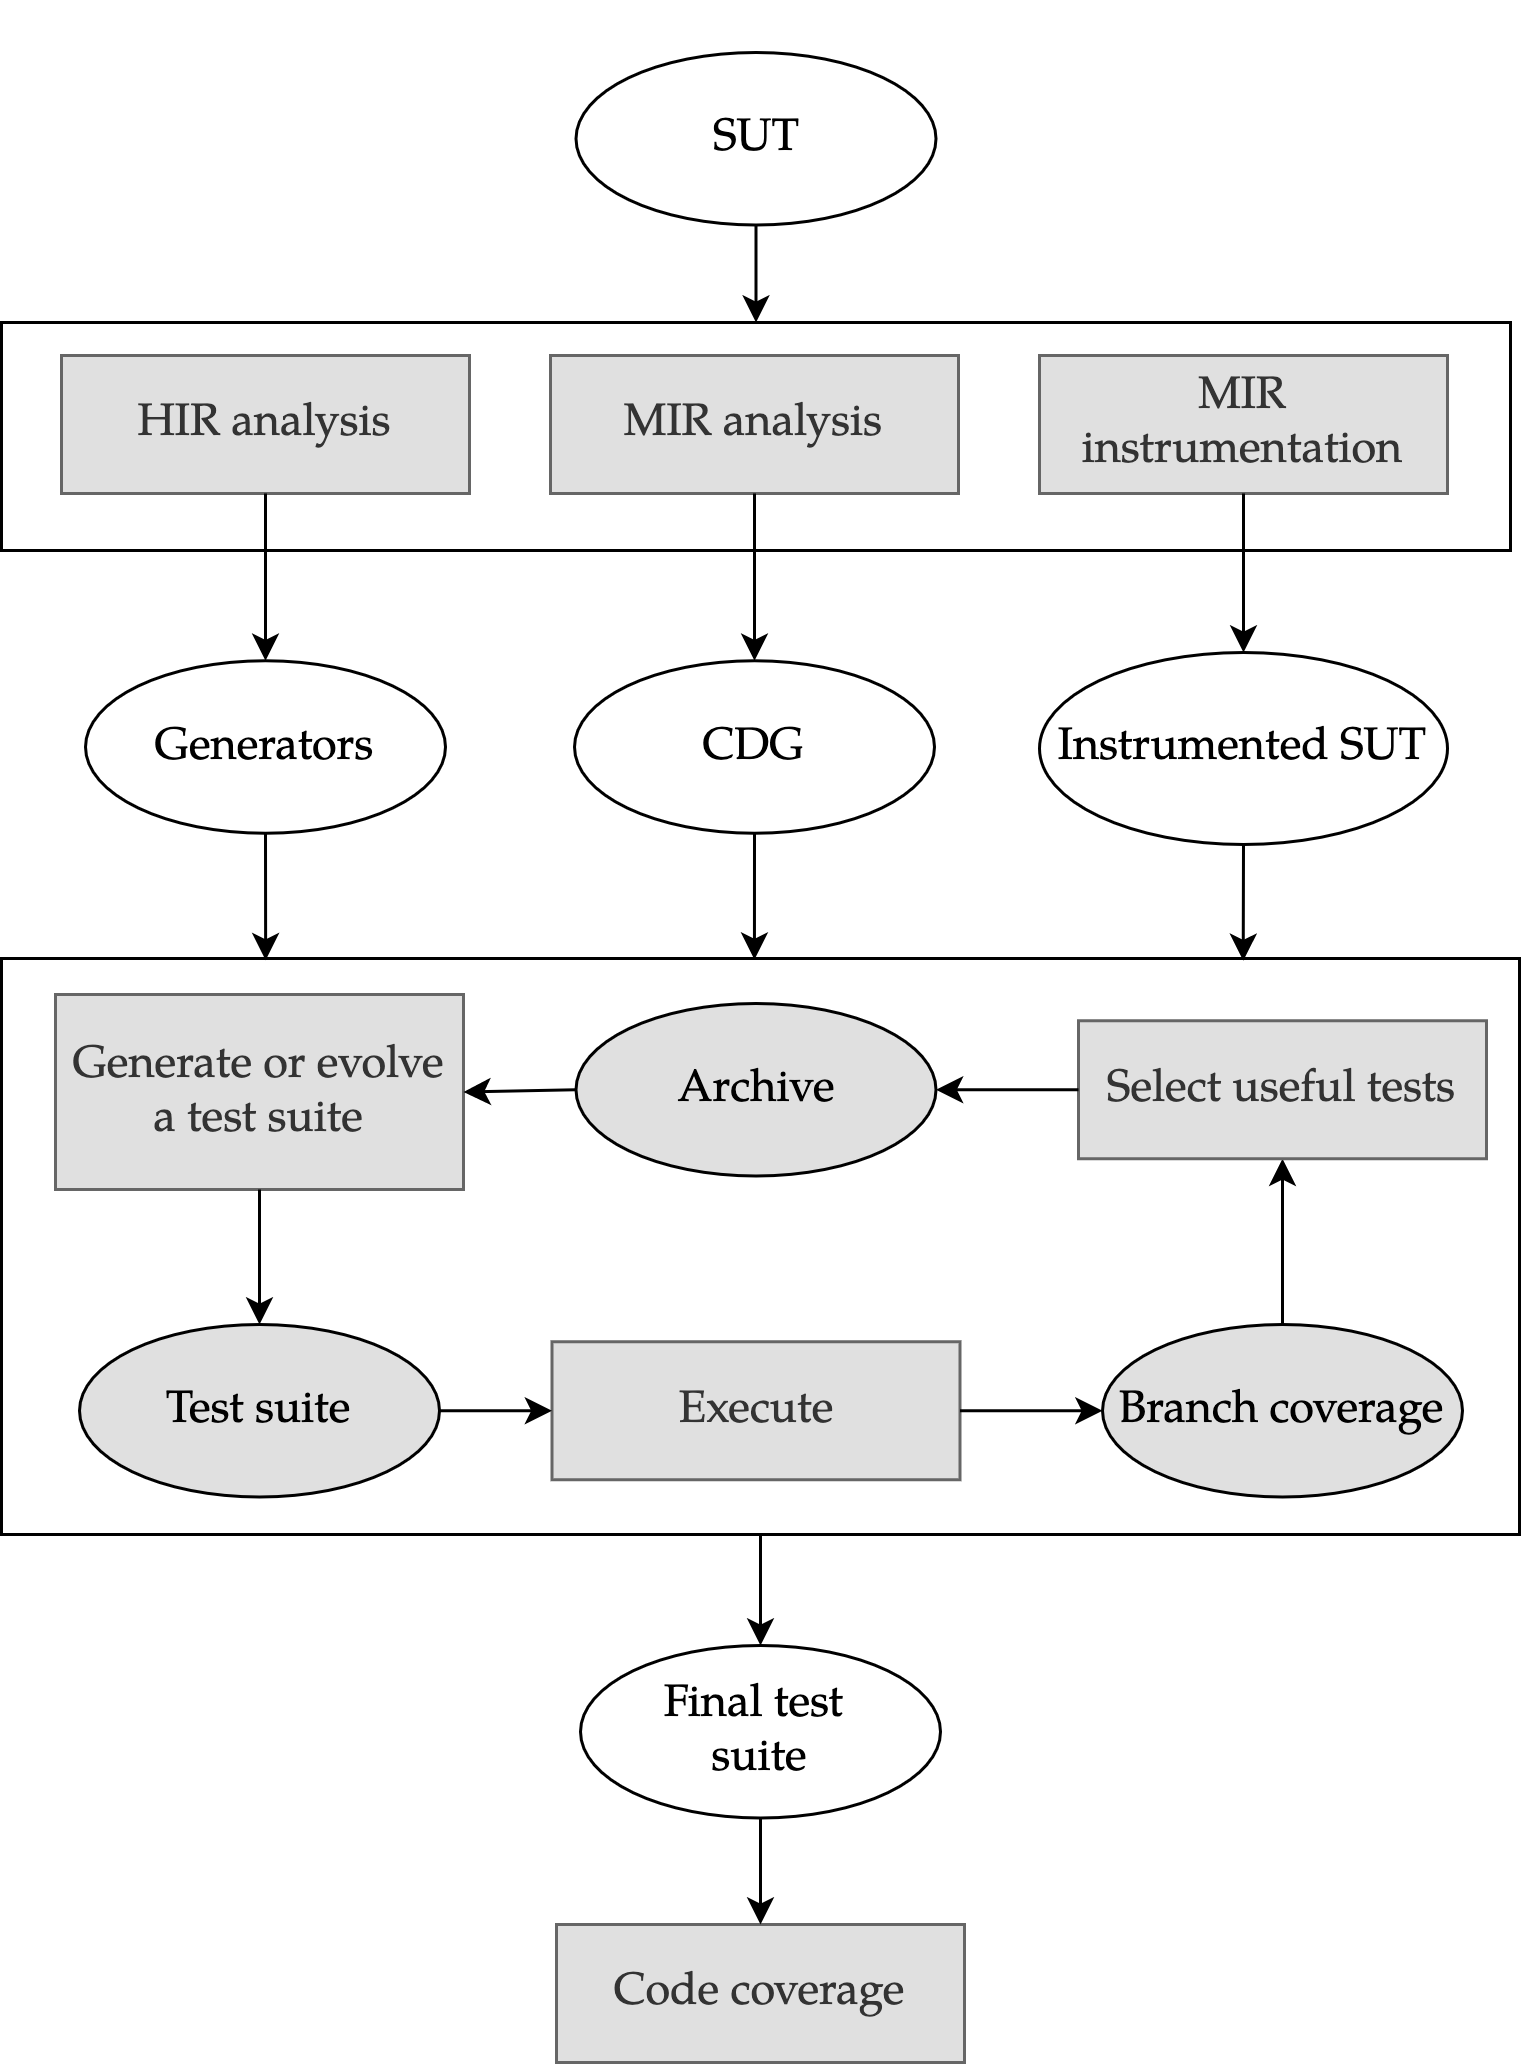
\includegraphics[width=\textwidth]{overview}
\label{fig:overview}
\end{figure}

\subsection{Problem representation}
%Laut McMinn~\cite{McMinn_2004} sollte eine Enkodierung der Lösung so gewählt sein, dass ähnliche Lösungen ebenfalls Nachbarn im repräsentierten Suchraum sind. Dadurch kann die Suche leicht von einer zur ähnlichen Lösung durch einfache Modifikationen der Repräsentation fortgeführt werden. In genetischen Algorithmen für Testgenerierung repräsentiert ein Chromosom in einer Population typischerweise eine ganze Testuite~\cite{Fraser_2011, Campos2017}. Fraser und Arcuri schlagen folgendes zu Repräsentation der Lösung vor~\cite{Fraser_2011}: Eine Lösung ist hier eine Test Suite~$T$, die im Grunde ein Set von Unit Tests ist und für welchen gilt: Wenn~$|T| = n$, dann~$T = \{t_1, t_2, ... ,t_n\}$. Ein Unit Test ist demnach eine Sequenz von Statements bzw. Programmaufrufen, die Teile des \ac{SUT} ausführen, um ein gewisses Objective (bzw. Branch) zu erreichen und abzudecken. Da Programme in Rust nicht nur Prozeduren sind, sondern eine bestimmte, Klassen-ähnliche Struktur haben, muss dies ebenfalls berücksichtigt werden. In einem einfachen prozeduralen Programm müssten Tests nur Prozeduren mit bestimmten Input-Daten aufrufen, um eine hohe Coverage zu erreichen. Instanzen von Klassen und (in Rust) Klassen-ähnlichen Structs können jedoch Zustände haben, die entweder direkt oder per Methodenaufrufe geändert werden können. Der Kontrollflussgraph einer Methode kann vom inneren Zustand eines Objekts abhängig sein. Das heißt, dass eine gewisse Statementaufrufsequenz von Bedeutung sein kann, um eine hohe Branch Coverage zu erreichen. Für die Generierung von Unit Tests mit einem genetischen Algorithmus werden in dieser Arbeit bereits bekannte Ideen für die Repräsentationen von genetischen Lösungen umgesetzt~\cite{Fraser2012,Tonella2004,Arcuri2008}.

According to McMinn~\cite{McMinn_2004}, an encoding of the solution should be modeled in a way that similar solutions are also neighbors in the represented search space. This makes it easy to continue the search from one to a similar solution by applying simple modifications of the representation. In single-objective genetic algorithms for test generation, a chromosome in a population typically represents an entire test suite~\cite{Fraser_2011, Campos2017}. However, \acp{MOA} define a chromosome to be a single test case~\cite{Panichella2018}. Chromosome representation has a direct impact on how, for instance, the crossover operator works. Recombining two test suites is trivial by recombining only the sequences of their test cases at specific cut points since individual test cases are independent of each other~\cite{Fraser_2013}. Recombining test cases is more complicated because it means recombining their sequences of statements, which are, however, very much interdependent. For example, a statement could instantiate an object by invoking an appropriate constructor, followed by a later method invocation on that object. In the following, a chromosome is a test case, which is a sequence of statements or program calls that execute parts of the \ac{SUT} to reach and cover a certain objective. Since programs in Rust are not just procedures but have a certain class-like structure, this must also be taken into account. In a simple procedural program, tests would only need to call procedures with certain input data to achieve high coverage. However, instances of classes and (in Rust) class-like structs can have states that can be changed either directly or via method calls. The control flow graph of a method may depend on the internal state of an object. This means that a certain statement call sequence may be important to achieve high code coverage. For the generation of unit tests with a genetic algorithm, this work implements already known ideas for the representations of genetic solutions~\cite{Fraser2012,Tonella2004,Arcuri2008}. Similar to Frasers and Arcuris~\cite{Fraser_2011} definition, each statement~$s_i$ in a test case is a value~$v(s_i)$, which can be of one of the following five types~$\tau(v(s_i))$: 
\begin{itemize} 
    \item \textbf{Primitive statements} represent numeric variables, e.g., \lstinline{let v = 42}.
    \item \textbf{Constructor statements} generate new instances of a given struct, z. B. \lstinline{let b = Book::new()}. A constructor can have parameters whose values are assigned out of the set ~$\{v(s_k)~|~0 \leq k < i\}$. However, constructors are not part of the Rust language. Using a static method called \lstinline{new}, which returns an instance of the appropriate struct, is not mandatory but a convention. Thus, if a struct does not provide the new method, it still can be instantiated the C-like way, i.e., \lstinline|let b = Book { name: "A" }|. 
    \item \textbf{Field statements} access member variables of objects, e.g., \lstinline{let b = a.x}. The source of the member variable, i.e.,~\lstinline{a}, must be part of the set~$\{v(s_k)~|~0 \leq k < i\}$. Since unit tests are usually contained in the same module as the~\ac{CUT}, tests can also legally access private fields and methods. 
    \item \textbf{Method statements} invoke associative methods on objects or static methods, e.g., \lstinline{let b = a.len()}. The owner of the method (if non-static) and all of the parameters must be values in~${\{v(s_k)~|~0 \leq k < i\}}$.
    \item \textbf{Function statements} invoke free-standing functions, e.g., \lstinline{let a = foo()}. The parameters of the function must be values in~$\{v(s_k)~|~0 \leq k < i\}$. 
\end{itemize}

%Die Sammlung von verfügbaren Structs, deren Konstruktoren, Methoden, Felder und frei stehende Funktionen sind ein sogenannter Test Cluster~\cite{Fraser_2011}. Die Größe einer Test Suite sowie einzelner Tests ist dabei dynamisch und kann sich (fast) beliebig verändern. Da für die meisten generierten Tests keine Testorakel zur Verfügung stehen werden, soll die Größe der Test Suite sowie der einzelnen Tests eine Obergrenze haben (kein Mensch möchte tausende Zeilen lange Tests durchlesen, um am Ende eine passende Assertion zu überlegen). 

The collection of available structs, their constructors, methods, fields, and free-standing functions are so-called test cluster~\cite{Fraser_2011}. The size of a test suite as well as individual tests is dynamic and can change (almost) arbitrarily. Since there will be no test oracles available for most of the generated tests, the size of the test suite, as well as the individual tests, should have an upper limit, so that test oracles can be inserted later manually. 

%Jedes Statement, welches nicht den default Rückgabewert~\lstinline{()} hat, definiert eine neue Variable. Ein generierter Test kann jedoch nicht beliebig aus den oben genannten Bausteinen zusammengesetzt werden. Er unterliegt den gleichen Constraints, wie reguläre Rust Programme, die vom Compiler überprüft werden~\cite{Tonella2004}. Konstruktoren, Methoden, Funktionen und Felder in einem Test sind nicht nur auf die Teile des Moduls unterm Test begrenzt, da für die Definition einiger Argumente komplexe Sequenzen von Aufrufen notwendig sein könnten~\cite{Fraser2012}. 

Each statement that does not have the default return value~\lstinline{()} defines a new variable. However, a generated test cannot be composed arbitrarily of the above building blocks. Each test is subject to the same constraints as regular Rust programs, which are checked by the compiler~\cite{Tonella2004}. Constructors, methods, functions, and fields in a test are not limited to just the parts of the module under the test since complex sequences of calls might be necessary to define some arguments~\cite{Fraser2012}. 

%Rusts affines Typsystem macht eine Wiederverwendung von bereits definierten Objekten komplizierter, da die Information, in welchen Aufrufen eine bestimmte Instanz auf welche Weise verwendet wurde (ausgeliehen oder konsumiert) ebenfalls mitgeführt werden muss. Das heißt, dass ein bereits definiertes Objekt nur dann von einem neu eingefügten Statement~$s$ verwendet werden darf, wenn es als frei verwendbar markiert ist und von keinem anderen Statement verwendet wird, das nach~$s$ kommt. Genauer werden die Regeln folgenderweise definiert: Sei~$t$ ein Test Case und $pos(s)$ eine Funktion, die die Position eines Statements~$s$ in der Sequenz von~$t$ zurückgibt. Sei~$o$ ein Objekt von einem Datentyp~$c$, das von einem Statement~$gen$ definiert wird. Ein neues Statement~$s'$ wird eingefügt, welches~$o$ verwendet. Es gilt für die Positionen:. Dann muss gelten:

Rust's affine type system makes usage of already defined objects more complicated since the information in which statements a particular instance was used in which way (borrowed or consumed) must also be tracked. That is, an already defined object may be used in any way by a newly inserted statement~$s'$ only if it is marked as free to use and is not used by any other statement~$s$ that comes after~$s'$. Otherwise,~$s'$ may use the object in a way that does not collide with~$s$. More precisely, the rules are defined as follows: let~$t$ be a test case and $pos(s)$ a function that returns the position of a statement~$s$ in the sequence of statements in~$t$. Let~$o$ be an object of a data type~$c$ defined by statement~$gen$. A new statement~$s'$ is inserted, which uses~$o$. Then the following must hold:
\begin{itemize}
    \item $gen \in t \wedge pos(gen) < pos(s')$.
    \item If~$o$ is not used by any statement~$s \in t$,~$o$ may be consumed or borrowed by~$s'$. 
    \item If~$o$ is borrowed by a statement~$s \in t$,~$o$ may also be borrowed by~$s'$ at position~$p_{borrow}$ with ~$pos(gen) < p_{borrow}$ or consumed at position~$p_{consume}$ with~$pos(s) < p_{consume} < \left|t\right|$. 
    \item If~$o$ is consumed by a statement~$s \in t$,~$o$ may be borrowed by~$s'$ at position~$p_{borrow}$ with~$pos(gen) < p_{borrow} < pos(s)$. 
\end{itemize}

Initialization and usage of objects shall be tracked in a \ac{DDG} per test case, e.g., as in Listing~\ref{lst:example-test}. The nodes in the graph are statements. When a statement~$a$ depends on some other statement~$b$, it means that~$a$ actually depends on a variable whose value has been defined by~$b$. 

\begin{minipage}{0.45\textwidth}
\begin{lstlisting}[language=Java, caption=An example test, label=lst:example-test]
let a = A::new();   // Id: stmt_a
let b = B::new(&a); // Id: stmt_b
let c = C::new();   // Id: stmt_c

a.foo(&b);          // Id: stmt_d
b.bar(c);           // Id: stmt_e
\end{lstlisting}
\end{minipage}%
\hfill
\begin{minipage}{0.45\textwidth}
\begin{figure}[H]
  \caption{The DDG of the example test}

  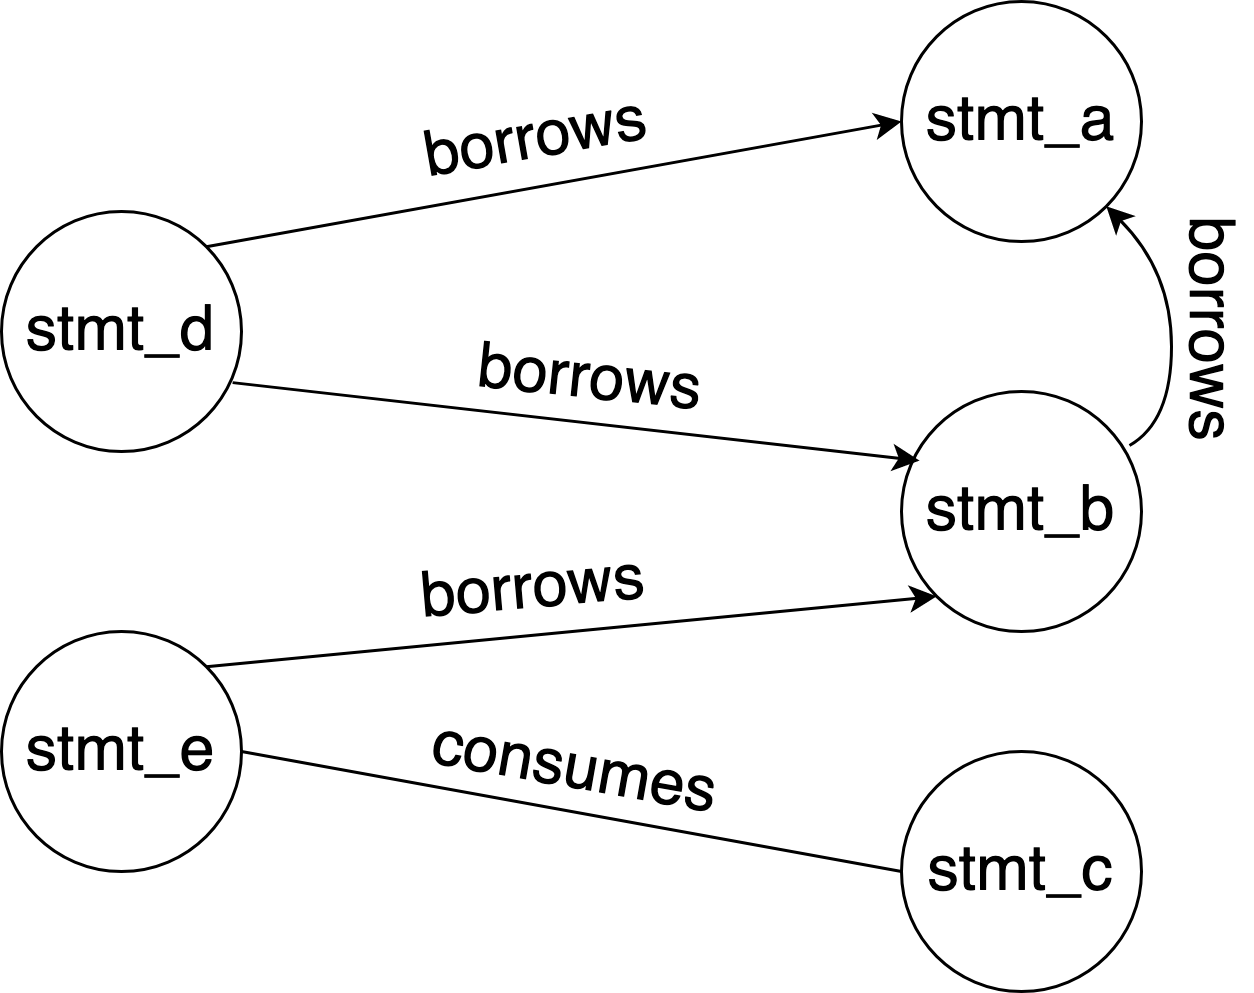
\includegraphics[width=\linewidth]{ddg-expose}
\end{figure}
\end{minipage}%

\subsection{Fitness Function}
%Eine gute Fitnessfunktion ist sehr wichtig bei der Suche nach Lösungen. Lösungen, die in einer bestimmten Weise \"besser\" als andere sind, sollen mit besseren Fitnesswerten belohnt werden~\cite{McMinn_2004}. Diese Arbeit hat die Branch Coverage im Fokus. Das Ziel ist es, die optimale Population von Lösungen zu finden, d. h. eine Test Suite, die möglichst hohe Branch Coverage hat. Gleichzeitig soll es aber keine andere Testsuite geben, die bei gleicher Branch-Coverage kleiner ist bzw. kleinere Tests enthält. Einige Branches, sogenannte infeasible Branches, können evtl. gar nicht abgedeckt werden, entweder aufgrund der limitierten Repräsentation der Lösung oder weil es keine passenden Inputs existieren, die allen Einschränkungen gerecht werden, z. B. $x < 4 \wedge x > 6$. Somit werden solche Tests bei der Optimierung der Lösung bevorzugt, die eine höhere Fitness bzgl. der Branch Coverage haben. Bei zwei Tests mit der gleichen Fitness wird der kürzere bevorzugt. 

There are different types of testing, e.g., temporal testing, functional testing, structural testing~\cite{McMinn2011}. Structural testing has seen the most attention in \ac{SBST}. Typically, a \ac{SUT} is instrumented and executed with inputs suggested by the search. The path taken through the program is then compared with some structure of interest for which coverage is sought~\cite{McMinn2011}. A good fitness function is important in the search for solutions for every type of testing. Solutions that are better than others in a certain way should be rewarded with better fitness values~\cite{McMinn_2004}. This approach targets structural testing, which most commonly is paired with branch coverage~\cite{McMinn2011} (however, statement coverage or mutation coverage are also possible~\cite{Korel1990}). The goal is to find an optimal population of solutions, i.e., a test suite that has the highest possible branch coverage. At the same time, there should be no other test suite that is smaller or contains smaller tests with the same branch coverage. Some branches, so-called infeasible branches, may not be covered at all, either because of the limited representation of the solution or because there are no suitable inputs that satisfy all constraints, e.g. $x < 4 \wedge x > 6$. Thus, tests that have a higher fitness with respect to the branch coverage are preferred when optimizing a solution. If two tests have the same fitness, the shorter one will be preferred in order to reduce the bloat. 

%Ein weitverbreitete Heuristik, um die Suche voranzutreiben, ist Branch Distance. Die Grundidee ist, dass wenn die Ausführung des \ac{SUT} bei gegebenen Inputdaten in einem bestimmten Branch landet, so kann eine lokale Suche angewendet werden. Es wird mit Hilfe einer lokalen Fitnessfunktion abgeleitet, wie nah ein Branch-Prädikat zum Auswerten zu \lstinline{true} oder \lstinline{false} ist. Zum Beispiel, bei einem Prädikat~\lstinline{x >= 10} und Inputdatum~\lstinline{x = 5} wird der \lstinline{false} Branch getroffen. Die Distanz zum \lstinline{true} Branch beträge somit~$10 - 5 + k$ mit~$k \geq 1$. Da jedes Prädikat im \ac{SUT} instrumentiert wird, können Distanzen zu anderen Branches während der Ausführung des \ac{SUT} getracet werden. Die Branch-Distanz muss noch normalisiert werden (je nach Werten kann es schnell zu Extremen kommen). Arcuri~\cite{Arcuri_2011} beschreibt in seiner Arbeit, welchen Einfluss die Normalisierung der Branch-Distanz auf die Effektivität einer such-basierten Testgenerierung hat. 

A popular fitness function used for guiding the search for test data to increase branch coverage incorporates two metrics, known as \textit{approach level} and \textit{branch distance}~\cite{Wegener2001}. The approach level is equivalent to the number of levels of conditional nesting left unpenetrated by the path to the target for structured programs. The branch distance is a measure of 'how close' an execution of a program with a certain input came to satisfying the condition of the predicate at which control flow went 'wrong', i.e., took the other branch. The idea is that if given some input data, the execution of a \ac{SUT} hits a particular branch, then a local search can be applied. A local fitness function~$d(b, t)$ is used to infer how close a branch predicate is to \lstinline{true} or \lstinline{false} for evaluation~\cite{McMinn_2004}. For example, given a predicate~\lstinline{x >= 10} and input data~\lstinline{x = 5}, the \lstinline{false} branch is hit. The distance to the \lstinline{true} branch is thus~$10 - 5 + k$ with~$k \geq 1$. As each predicate is instrumented in the \ac{SUT}, distances to other branches can be traced during the execution. For \ac{DynaMOSA}, the coverage criterion is defined as follows: \textit{Let $B = \{b_1, ..., b_k\}$ be the set of branches to cover. Find a set of non-dominated test cases $T = \{t_1,...,t_n\}$ that minimizes the fitness functions for all branches $b_1, ..., b_k$, i.e., minimizing the following k objectives:}
\[
     \left\{\begin{array}{l}
         \text{min}f_1(t) = al(b_1,t) + d(b_1,t)\\
         . \\
         . \\
         \text{min}f_k(t) = al(b_k,t) + d(b_k,t)
        \end{array}
    \right.
  \]
\textit{where each $d(b_j, t)$ denotes the branch distance for the branch, executed by $t$, which is closest to $b_j$ (i.e., which as at minimum number of control dependencies from $b_j$), while $al(b_j,t)$ is the corresponding approach level (i.e., the number of control dependencies between the closest executed branch and $b_j$).}
%The branch distance still needs to be normalized (depending on values, extremes can quickly occur). Arcuri~\cite{Arcuri_2011} describes in their work which impact the normalization of the branch distance has on the effectiveness of~\acp{GA}. 
%The lower the distance to a branch, the better, i.e., the minimum fitness value is 0 when a branch is hit. However, the maximum value is technically unbounded, which can result in huge values. Arcuri~\cite{Arcuri_2011} shows in their work 


\subsection{Suchoperatoren}
The evolution of a population is performed by repeated selection of test cases and applying crossover and mutation operators according to a certain probability~\cite{Fraser2012}.

There are different selection methods, e.g., fitness-proportional selection, linear ranking, or tournament selection~\cite{McMinn_2004}. The key is to guide the search towards solutions with better fitness values. Once the set of parents has been selected, recombination (or crossover) can take place to form the next generation. Crossover is applied to individuals with a certain probability. The most basic recombination is a single point crossover, where a random position in each of the two selected test cases is selected, and new test cases (offspring) are generated by swapping the subsequences of statements~\cite{Fraser2012}. At this point, the dependencies of the statements will be considered, and possibly missing arguments will be generated in the offspring test cases. In addition, the \acp{DDG} of those test cases must also be adjusted.

After selection and crossover have been applied, the offspring can mutate. There are different ways of mutation, e.g., delete, insert, or modify a statement~\cite{Fraser2012}. Modifying a statement includes changing the callee of a method, parameters, or replacing the method itself with another one. The \ac{DDG} of each test case determines what mutation is possible, e.g., replacing a method call to \lstinline{fn foo(&self)} by \lstinline{fn bar(self)} is not allowed if the callee of the method is also used by some other statement later in the sequence because the \lstinline{bar} method consumes the callee. 


\subsection{Instrumentation}
Beschreibung zur Insrumentierung und Setup~\cite{Fraser2012}

Tests that are generated by a search-based technique need to be executed at least once to provide some feedback on their fitness in regard to the \ac{SUT}. At this point, the coverage data and branch distances can be collected. In order to do so, the \ac{SUT} has to be instrumented with additional code, which traces the executed paths. Many other state of the art tools that generate coverage for Java instrument the bytecode of the compiled \ac{SUT} and use Reflection to run the generated tests. However, Rust compiles to machine code. Although there exist tools that allow static analysis and binary transformation, e.g., reg.ng~\cite{DiFederico2018}, the instrumentation will be done on the source code level. \textbf{syn} and \textbf{quote} are two mature libraries that allow parsing Rust code into a syntax tree and converting the tree back to regular code, respectively. 

During the instrumentation, additional tracing statements will be inserted into a \ac{SUT} to report visited branches. The original source files will be backed up and temporarily replaced by the instrumented ones. Additionally, while traversing the syntax tree, all testable data structures, as well as their constructors, fields, and methods, are captured. At the end of this process, it will be known which methods can be tested, what parameters they have, which generators can be used to instantiate those parameters, and how the parameters are used, i.e., borrowed or consumed. 

\subsection{Test Oracles and Testability Transformations}
Traditionally, \ac{SBST} is applied to generate test suites that maximize some coverage criteria, e.g., in this case, branch coverage. However, search-based techniques usually do not make any use of automated oracles~\cite{Fraser2013}. A lack of formal specification of the behavior of a program results in generated tests that must be supplemented with oracles manually. A technique called \textit{testability transformation} tries to overcome this obstacle. A testability transformation is a source-to-source program transformation that seeks to improve the performance of some chosen test data generation technique~\cite{Harman2004}, e.g., reach difficult branches. Beyond that, a \ac{SUT} can be transformed in a way such that artificial branches are inserted into the code to guide the search into triggering some exceptional behavior and crash the program. For instance, EvoSuite~\cite{Fraser2013} employs multiple testability transformations such as array access transformation, division by zero transformation, or numerical overflow transformation. Those transformations do not increase code coverage in general but contribute to discovering potential unforeseen behavior and generating inputs that trigger it. Similar transformations can also be applied for Rust and shall be part of the approach.

\subsection{Test Execution}
%Mit Cargo bringt Rust automatisch auch ein Build System und ein Testing Framework. In Java, which is a managed language~\cite{Gough2005}, können generierte Tests mittels Reflection und Instrumentierung direkt ausgeführt und Coverage von Tests im gleichen Laufzeitprozess collected werden. Das geht in Rust nicht so bequem, und Tests müssen erst kompiliert werden. Danach wird das Cargo Test Framework auf dem zu testenden Modul aufgerufen, um Tests laufen zu lassen. Um den Prozess zu beschleunigen wird jeweils die ganze Population von Tests kompiliert und concurrently laufen gelassen. Um die genaue Coverage eines jeden einzelnen Tests zu behalten, setzt jeder Test am Anfang seiner Ausführung eine \lstinline{thread_local} ID, die das instrumentierte \ac{SUT} bei der Ausführung verwendet, um die Coverage zu tracen. 

With Cargo, Rust provides a build system and a testing framework out-of-the-box. In Java, which is a managed language~\cite{Gough2005}, generated tests can be executed directly using Reflection and bytecode instrumentation, and coverage information can be collected in the same runtime process. This cannot be done that conveniently in Rust, and tests must first be compiled. Then the Cargo test framework is called on the module under test to run the tests. To speed up the process, a whole population of tests is compiled and run concurrently. To keep the exact coverage of each individual test, each test sets a \lstinline{thread_local} ID at the beginning of its execution, which the instrumented \ac{SUT} uses during execution to trace the coverage. 

%Wie in Figure~\ref{fig:test-execution} dargestellt, reportet das instrumentierte \ac{SUT} die wichtigen Ereignisse bei seiner Ausführung an die Message Queue des Monitor Threads (MT). Diese sind zum Beispiel das Ausführen eines Root Branches (Methode oder Funktion) oder eines Decision Branches. Beim letzteren wird direkt die bei der Ausführung berechnete Branch Distanz zum anderen Branch übergeben. Der MT wird vor dem Starten der Threads initialisiert und kann gesammelte Coverage Daten entweder in eine Datei schreiben oder per TCP an den Hauptprozess direkt senden.

As shown in Figure~\ref{fig:test-execution}, the instrumented \ac{SUT} reports important events during its execution to the message queue of the monitor thread (MT). These are, for example, the execution of a root branch (method or function) or a decision branch. For the latter, the branch distance, which is calculated on the fly, is passed along with other data. The MT is initialized before the threads are started and can either write collected coverage data to a file or send it directly to the main process via TCP.

\begin{figure}[h]
\caption{An example concurrent execution of multiple tests with a monitor}
\centering
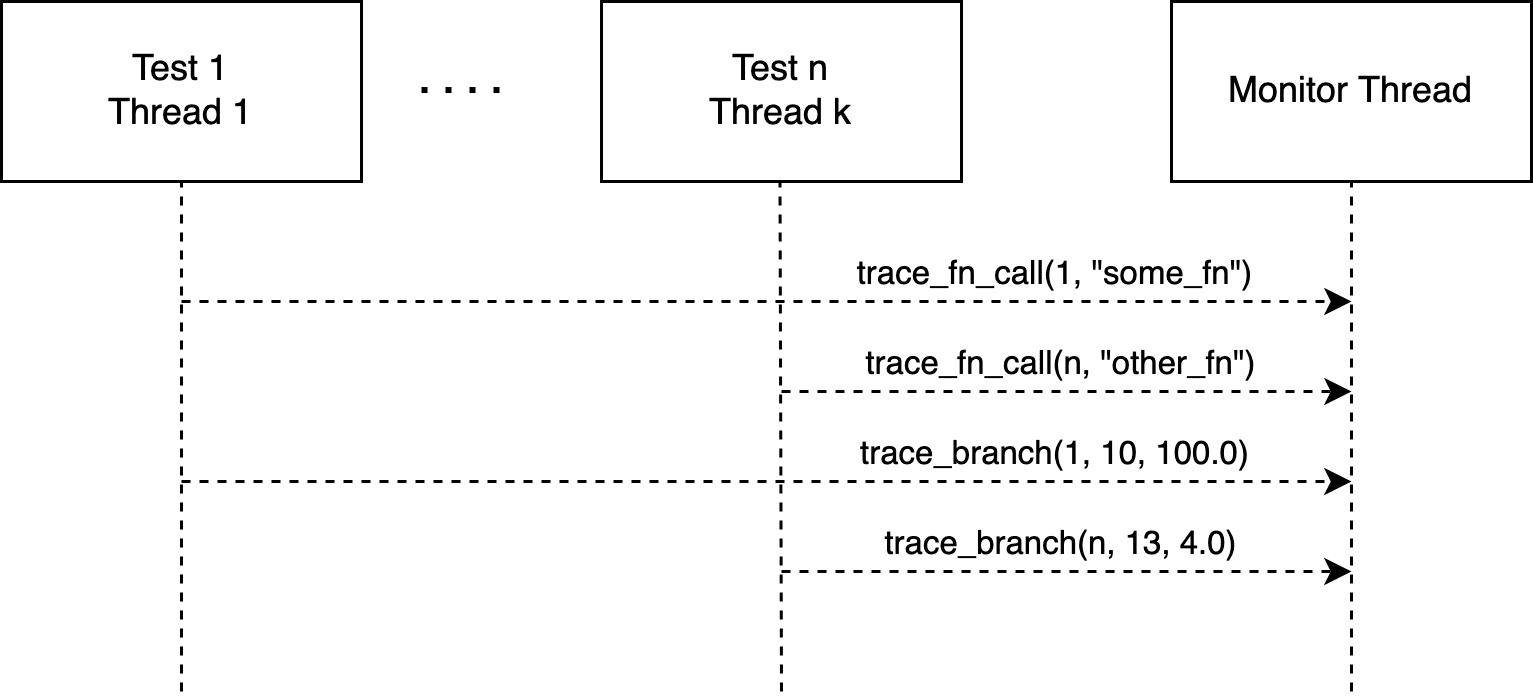
\includegraphics[width=\textwidth]{test-execution}
\label{fig:test-execution}
\end{figure}

%Echte und komplexe Software interagiert oft mit ihrer Umgebung, in dem zum Beispiel I/O Aufrufe zum Filesystem ausgeführt werden oder TCP Verbindungen aufgebaut werden. Um unerwünschte Seiteneffekte zu vermeiden, greift EvoSuite~\cite{Fraser2013a} auf strenge Sicherheitsmaßnahmen des Java Security Managers zürück und verbietet die meisten Interaktionen des \ac{SUT} mit seiner Umgebungen. Diese könnten bei wiederholten Ausführungen zu unkontrolliertem Verhalten führen, wie zum Beispiel Generieren von unzähligen zufälligen Dateien oder gar Löschen der gesamten Festplatte. Nur ganz wenige essentielle Operationen werden gestattet, wie zum Beispiel I/O für den Classloader, das Laden von Libraries oder Reflection. 

Real and complex software often interacts with its environment, for example by making I/O calls to the file system or establishing TCP connections. Lack of handling of the execution environment the \ac{SUT} lives within is still one of the open problems in \ac{SBST}~\cite{McMinn2011}. To avoid unwanted side effects, EvoSuite~\cite{Fraser2013a} relies on strict security measures of the Java Security Manager and prohibits most interactions of \ac{SUT} with its environments. These could lead to uncontrolled behavior if executed repeatedly, such as generating countless random files or even wiping the entire disk. Only a very few essential operations are allowed, such as I/O for the classloader, loading libraries, or reflection. As a preprocessing step, EvoSuite extracts only those methods that return the same result when run repeatedly with the same inputs, i.e., methods that are deterministic~\cite{Fraser2012}.

%KLEE~\cite{cadar2008klee} geht an dieser Stelle einen anderen Weg und redirects konkrete Aufrufe, wie zum Beispiel \lstinline{open()} und \lstinline{read()}, zu \textit{models} that understand the semantics of the desired action well enough to generate the required constraints. These models are written in normal C code which the use can readily customize, extend, or even replace with their own custom implementation. Ein ähnliches Verfahren soll auch in dieser Arbeit angewendet werden. Funktionsaufrufe sollen in einem Pre-Processing Schritt im \ac{SUT} durch Mocks ersetzt werden, die das ursprüngliche Verhalten nachahmen. Wenn das \ac{SUT} Werte aus der Umgebung liest, wie zum Beispiel aus einer Datei, soll ein legaler, zufällig generierter Wert des gleichen Typs zurückgegeben werden, wie es die originale Funktion getan hätte. Wenn das \ac{SUT} schreibend auf die Umgebung zugreift, sollen die Werte während der Ausführung des entsprechenden Tests in Memory gespeichert werden so the effect of these alterations should be reflected in potential subsequent reads.

KLEE~\cite{cadar2008klee} takes a different approach and redirects concrete calls, such as \lstinline{open()} and \lstinline{read()}, to \textit{models} that understand the semantics of the desired action well enough to generate the required constraints. These models are written in normal C code which the use can readily customize, extend, or even replace with their own custom implementation. Function calls are replaced in a pre-processing step in \ac{SUT} by mocks that mimic the original behavior. When the \ac{SUT} reads values from the environment, such as from a file, a legal, randomly generated value of the same type is returned as the original function would have done. When the \ac{SUT} writes to the environment, the values are stored in memory during the execution of the corresponding test such that the effect of these alterations are reflected in potential subsequent reads. 

\subsection{Test Minimization}
%Da sich diese Arbeit vor allem auf das Generieren vor Tests beschränkt, die möglichst hohe Coverage erreichen, jedoch generell keine Testorakel automatisch zur Verfügung stellt, sollen die Tests möglich kurz gehalten werden und das wesentliche tun, um einen bestimmten Branch zu erreichen. Das erhöht ihre Lesbarkeit und Verstänlichkeit. Fraser und Arcuri~\cite{Fraser2013a} schlagen als Verbesserung für ihr EvoSuite Tool folgendes Verfahren vor: Für jeden Coverage Goal wird ein Test aus der generierten Test Suite ausgewählt, der diesen Goal abdeckt. Dieser Test wird wrt to the coverage goal minimiert, so dass Statements, die nicht zur Ausführung des Goals beitragen, gelöscht werden. Wenn ein Goal bereits von einem minimierten Test abgedeckt ist, so wird kein weiterer Test für diesen Goal der finalen Test Suite hinzugefügt. Auf diese Weise werden Tests lesbarer für einen Menschen und können somit leichter manuell um Testorakel ergänzt werden. 

Since this work is mainly limited to generating tests that achieve the highest possible coverage but do not provide test oracles automatically in general, the tests should be kept as short as possible and do the essential to achieve a certain branch. This increases their readability and comprehensibility. Fraser and Arcuri~\cite{Fraser2013a} propose the following procedure as an improvement for their EvoSuite tool: for each coverage goal, a test is selected from the generated test suite that covers that goal. That test is minimized with respect to the coverage goal so that statements that do not contribute to the execution of the target are removed from the test. If a target is already covered by a minimized test, no further test for this objective will be added to the final test suite. This way, tests become more readable to a human and can thus be more easily supplemented manually with test oracles. 

\section{Evaluation}
To determine how well a search-based approach performs with respect to code coverage and program crash detection, a set of experiments shall be conducted on a set of open-source Rust software. As there is already another tool available, KLEE, which uses \ac{DSE} and can also generate tests for Rust, it can be used in the experiments. KLEE-generated tests do not depend on the tool itself and can be executed outside of it the usual way. This opens the possibility to compute a source-based code coverage available in the Rust compiler for both tools. The experiments should answer the following questions: 

%Symbolic execution often has problems constructing nice test suites with complex types, which is why this technique is rather applied to find bugs in a \ac{SUT}, than generate tests with high coverage. Seach-based approach do the opposite, they are good at generating tests with high coverage, but are not as good at finding bugs as they do not make use of test oracles~\cite{Fraser2013}.

\begin{enumerate}[start=1, label={\bfseries RQ\arabic*:}]
    \item How many program crashes and generic contact violations can be found with \ac{SBST} in open source Rust software?
    \item Does an \ac{SBST} approach achieve a higher code coverage than a \ac{DSE}-based one?
    \item Does an \ac{SBST} approach achieve a higher code coverage than manually written tests in open-source Rust software?
\end{enumerate}
To this end, a set of real Rust programs shall be chosen for experiments. The programs for experiments must comply with the following prerequisites:
\begin{itemize}
    \item There is no concurrency involved, as it introduces non-determinism and flakiness in the tests.
    \item The programs do not make use of \textit{unsafe} Rust and do not depend on external bindings, e.g., to C or C++.
    \item The programs do not interact with the execution environment, e.g., open read or write files.
    \item The programs already contain a manually written test suite that can be used in the evaluation to compare the coverage of the generated tests. 
    \item The programs use only \textit{stable} language features of Rust.
\end{itemize}


\appendix
\chapter{Acronyms}
\begin{acronym}
	\acro{SUT}{System Under Test}
	\acro{CUT}{Class Under Test}
	\acro{MUT}{Method Under Test}
	\acro{SMT}{Satisfiability Modulo Theories}
	\acro{GA}{Genetic Algorithm}
	\acro{EA}{Evolutionary Algorithm}
	\acro{MOSA}{Many-Objective Sorting Algorithm}
	\acro{DynaMOSA}{Many-Objective Sorting Algorithm with Dynamic target selection}
	\acro{WS}{Whole Suite}
	\acro{WSA}{Whole Suite with Archive}
	\acro{SBST}{Search-based Software Testing}
	\acro{SBSE}{Search-based Software Engineering}
	\acro{ATP}{Automated Theorem Prover}
	\acro{DSE}{Dynamic Symbolic Execution}
	\acro{IR}{Intermediate Representation}
	\acro{MOA}{Multi- and Many-Objective Algorithm}
	\acro{DDG}{Data Dependence Graph}
	\acro{HIR}{High-level Intermediate Representation}
	\acro{THIR}{Typed HIR}
	\acro{MIR}{Mid-level Intermediate Representation}
	\acro{AST}{Abstract Syntax Tree}
	\acro{CFG}{Control Flow Graph}
	\acro{CDG}{Control Dependence Graph}
	\acro{API}{Application Programming Interface}
	\acro{NSGA-II}{Non-dominated Sorting Genetic Algorithm II}
	\acro{TCP}{Transmission Control Protocol}
	\acro{SSA}{Static Single Assignment}
\end{acronym}

\bibliographystyle{unsrt}
\bibliography{bibliography}
%\nocite*{}
\end{document}